\documentclass[UTF8,12pt]{article}
\usepackage{ctex}
\usepackage{indentfirst}
\usepackage{color}
\usepackage{hyperref}
\usepackage{graphicx}
\usepackage{subfigure}
\usepackage{pdfpages}
\usepackage{listings}
\hypersetup{
    hidelinks,
	colorlinks=true,
	allcolors=black,
	pdfstartview=Fit,
	breaklinks=true
}

\definecolor{dkgreen}{rgb}{0,0.6,0}
\definecolor{gray}{rgb}{0.5,0.5,0.5}
\definecolor{mauve}{rgb}{0.58,0,0.82}

\lstset{ %
  language=Octave,                % the language of the code
  basicstyle=\footnotesize,           % the size of the fonts that are used for the code
  numbers=left,                   % where to put the line-numbers
  numberstyle=\tiny\color{gray},  % the style that is used for the line-numbers
  stepnumber=2,                   % the step between two line-numbers. If it's 1, each line 
                                  % will be numbered
  numbersep=5pt,                  % how far the line-numbers are from the code
  backgroundcolor=\color{white},      % choose the background color. You must add \usepackage{color}
  showspaces=false,               % show spaces adding particular underscores
  showstringspaces=false,         % underline spaces within strings
  showtabs=false,                 % show tabs within strings adding particular underscores
  frame=single,                   % adds a frame around the code
  rulecolor=\color{black},        % if not set, the frame-color may be changed on line-breaks within not-black text (e.g. commens (green here))
  tabsize=2,                      % sets default tabsize to 2 spaces
  captionpos=b,                   % sets the caption-position to bottom
  breaklines=true,                % sets automatic line breaking
  breakatwhitespace=false,        % sets if automatic breaks should only happen at whitespace
  title=\lstname,                   % show the filename of files included with \lstinputlisting;
                                  % also try caption instead of title
  keywordstyle=\color{blue},          % keyword style
  commentstyle=\color{dkgreen},       % comment style
  stringstyle=\color{mauve},         % string literal style
  escapeinside={\%*}{*)},            % if you want to add LaTeX within your code
  morekeywords={*,...}               % if you want to add more keywords to the set
}


\setlength{\parindent}{2em}

\begin{document}

\begin{titlepage}
    \includepdf[pages={1}]{cover.pdf}
\end{titlepage}

\begin{center}
    \tableofcontents
\end{center}
\newpage

\section{问题描述}
\subsection{实践目的}
通过指导学生上机实践,让学生学会综合运用所学过的《计算机程序设计基础》、《数据结构》、《算法》、《Java语言与系统设计》、《数据库》、《Web技术》、《移动应用开发》等课程的基础知识,从而能够熟练掌握开发市面上比较流行的移动应用开发的基本技能,设计和开发出具有一定规模的Android客户端应用+JSP(PHP)服务器端编程+MySQL数据库的典型移动互联网应用。

\subsection{课程设计的基本要求}
\begin{itemize}
    \item 知识:了解HTML、HTML5、CSS、JavaScript、JSP、Android等开发技术在实际移动互联网应用开发过程中的基本用法;
    了解移动互联网应用开发从需求分析、系统设计、模块设计、开发以及调试的各个环节。
    掌握典型移动互联网应用各个环节的技术以及具体运用方式;
    了解移动互联网典型应用开发是如何结合Web相关技术(HTML、HTML5、CSS、JavaScript、JSP等)、移动客户端开发技术(Android为例)以及数据库技术(以MySQL为例)进行开发的。
    \item 能力:通过从无到有动手完成基于Web+Android+MySQL移动应用开发的案例的设计、编码和调试工作,将对移动互联网应用开发的理性认识转变为感性认识,
    初步体会和理解计算机相关学科的软件项目工程的具体概念,体会工程的复杂性;学会将理论知识与实际生产结合,学会用工程的角度去提出问题、分析问题和解决问题;
    初步建立移动互联网应用软件工程开发项目需求分析、总体设计、模块设计、编码实现和调试的完整概念,提高实际动手能力,
    为具备大型移动互联网应用开发软件系统从设计到开发的能力打下坚实基础。
    \item 素质:通过实际动手设计和开发多个完整的移动互联网应用实例,培养理论知识的综合运用能力和动手编程开发的能力,培养软件工程开发的流程化管理观念;在实习中理解并遵守软件工程开发的职业道德和规范,履行责任,提高职业规范素质。
\end{itemize}

\subsection{项目基本内容与要求}
\begin{enumerate}
    \item 用Android开发看病预约客户端
    \item 用JSP或PHP开发预约挂号Web服务器的后台数据库
    \item 用MySQL做预约挂号Web服务器的后台数据库
    \item 可以预约挂号、查看医生介绍及日程安排列表等功能
    \item 可以实现患者注册、登录功能
    \item 在线挂号支付
\end{enumerate}

\newpage

\section{需求分析}
\subsection{开发环境}
\begin{itemize}
    \item 数据库
    \\集成环境:Navicat Premium 16
    \\MySQL 5.7.31
    \item Web服务器
    \\集成环境:Intellij IDEA 2023.1.4
    \\JDK 17.0.4.1
    \\Tomcat 9.0.55
    \item Android客户端
    \\集成环境:Android Studio 2022.3.1
    \\Android SDK 31.0.0
\end{itemize}

\subsection{用例分析}
本应用作为医院的看病预约应用

主要的actor是患者


主要的use case包括以下几个:
\begin{itemize}
    \item 患者注册
    \item 患者登录
    \item 患者预约挂号
    \begin{itemize}
        \item 患者选择科室
        \item 患者选择医生
        \item 患者选择预约时间
        \item 患者在线支付
        \item 患者查看医生介绍
    \end{itemize}
    \item 患者查看自己的预约挂号
\end{itemize}

\begin{figure}[htbp]
    \centering
    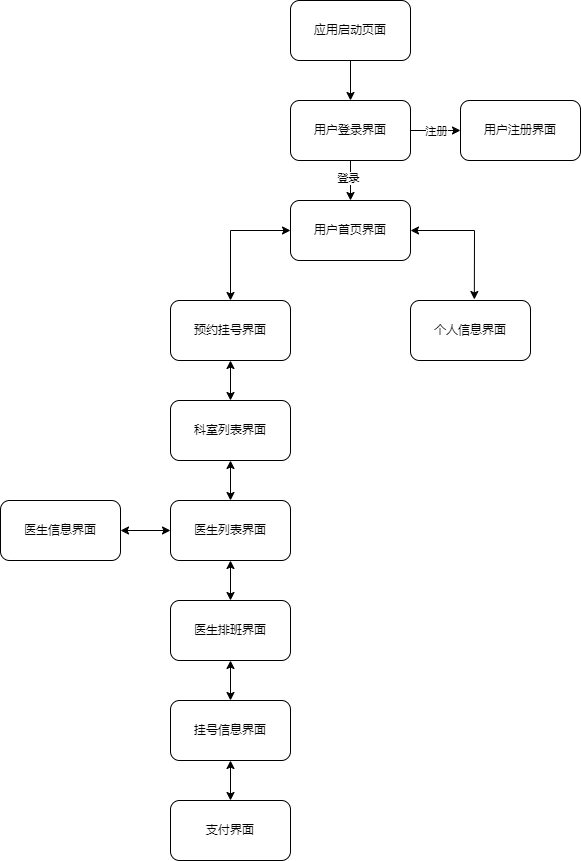
\includegraphics[width=0.6\textwidth]{imgs/1.png}
    \caption{看病预约应用用例图}
\end{figure}



\newpage

\section{设计思想}

\newpage

\section{概要设计}

\subsection{数据库概要设计}
新建数据库并命名为hospital,数据库的结构如下

\begin{lstlisting}[frame=shadowbox]
+--------------------+
| Tables_in_hospital |
+--------------------+
| depart             |
| doctor             |
| myorder            |
| schedule           |
| user               |
+--------------------+
\end{lstlisting}

五个表中的作用如下:

\begin{itemize}
    \item user表:存储用户相关信息
    \item depart表:存储科室相关信息
    \item doctor表:存储医生相关信息
    \item schedule表:存储医生的排班信息
    \item myorder表:存储用户的预约挂号信息
\end{itemize}

\newpage

\section{详细设计}

\subsection{数据库详细设计}

\subsubsection{user表}
user表的主要字段有uid,uname,upsw,分别代表用户id,用户名,密码

\newpage

\begin{figure}[htbp]
    \centering
    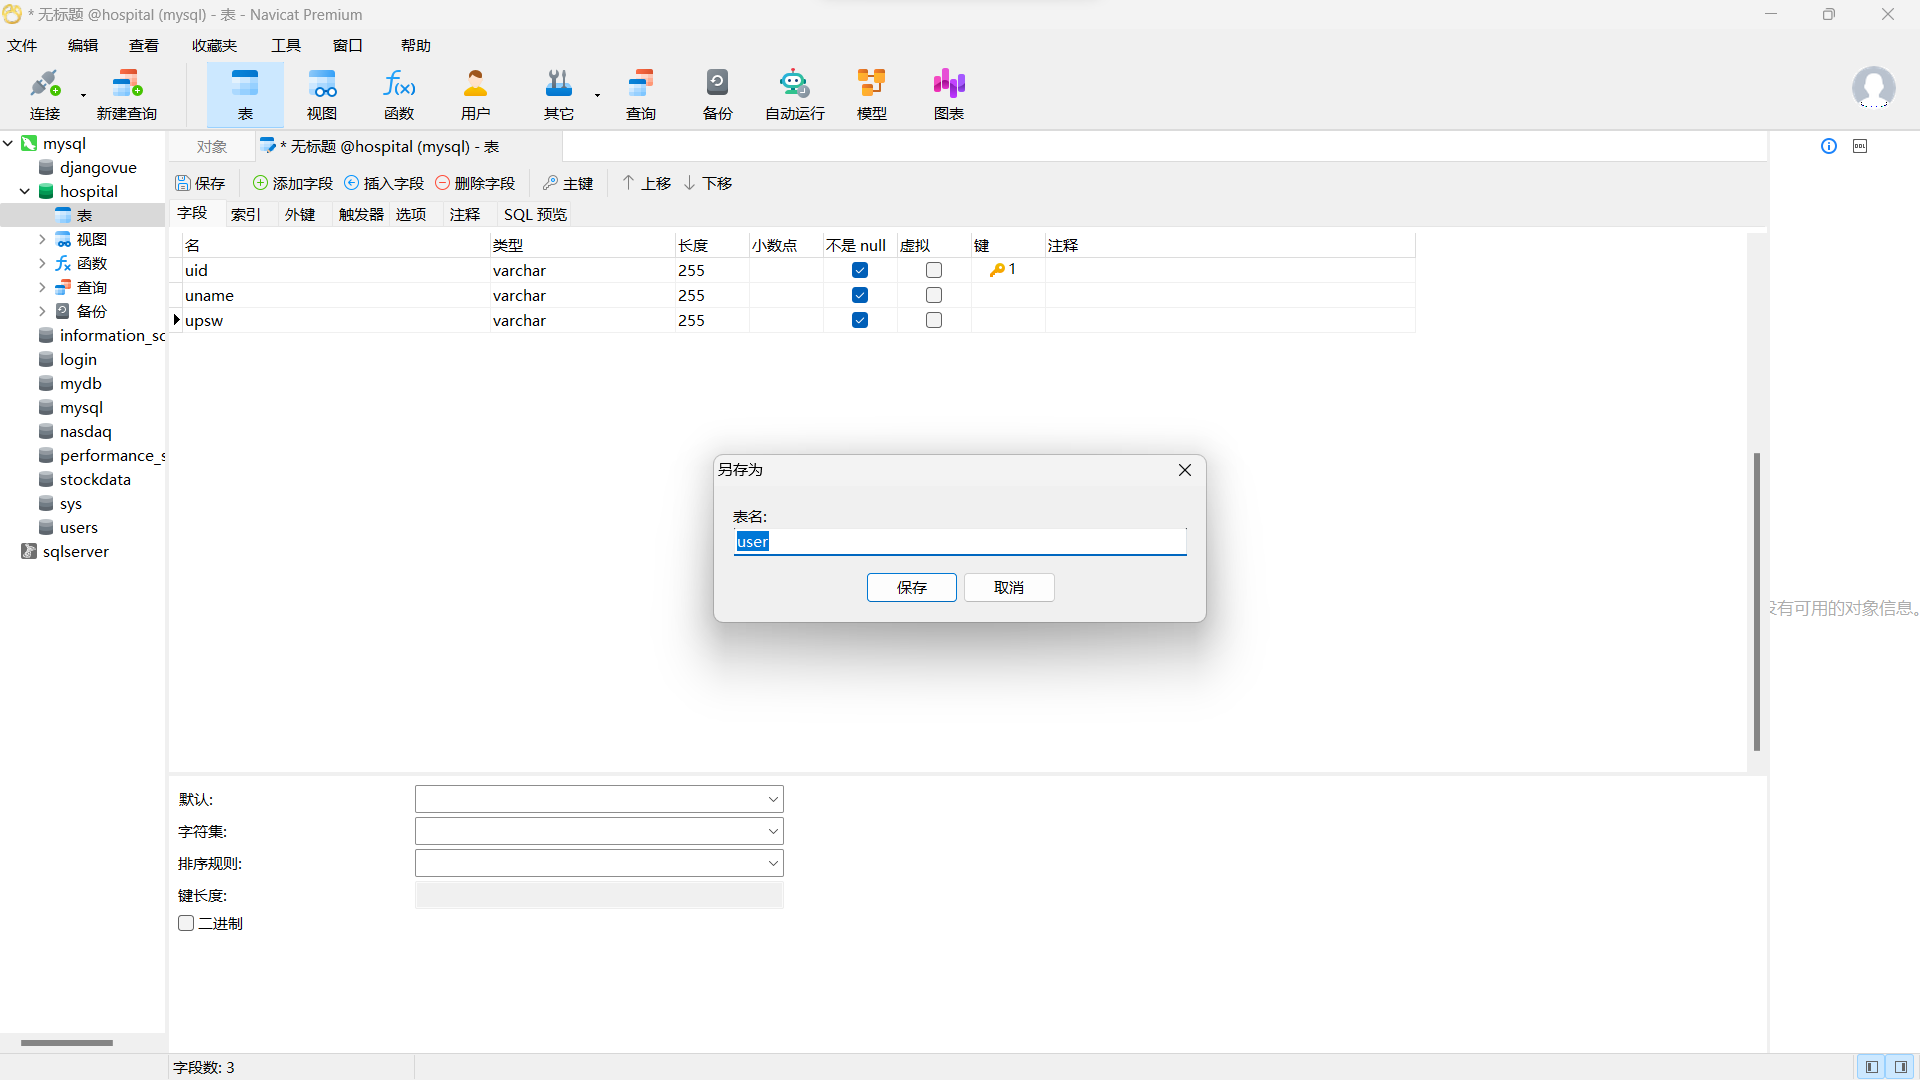
\includegraphics[width=0.6\textwidth]{imgs/5.png}
    \caption{user表}
\end{figure}

设计出的table结构如下

\begin{lstlisting}[frame=shadowbox]
+-------+--------------+------+-----+---------+-------+
| Field | Type         | Null | Key | Default | Extra |
+-------+--------------+------+-----+---------+-------+
| uid   | varchar(255) | NO   | PRI | NULL    |       |
| uname | varchar(255) | NO   |     | NULL    |       |
| upsw  | varchar(255) | NO   |     | NULL    |       |
+-------+--------------+------+-----+---------+-------+
\end{lstlisting}

\subsubsection{doctor表}

doctor表的主要字段有did,dname,dlevel,dinfo,departid,sex,ddetail分别代表医生id,医生姓名,医生职级,医生简介,医生所属科室id,医生性别,医生详细信息

\newpage

\begin{figure}[htbp]
    \centering
    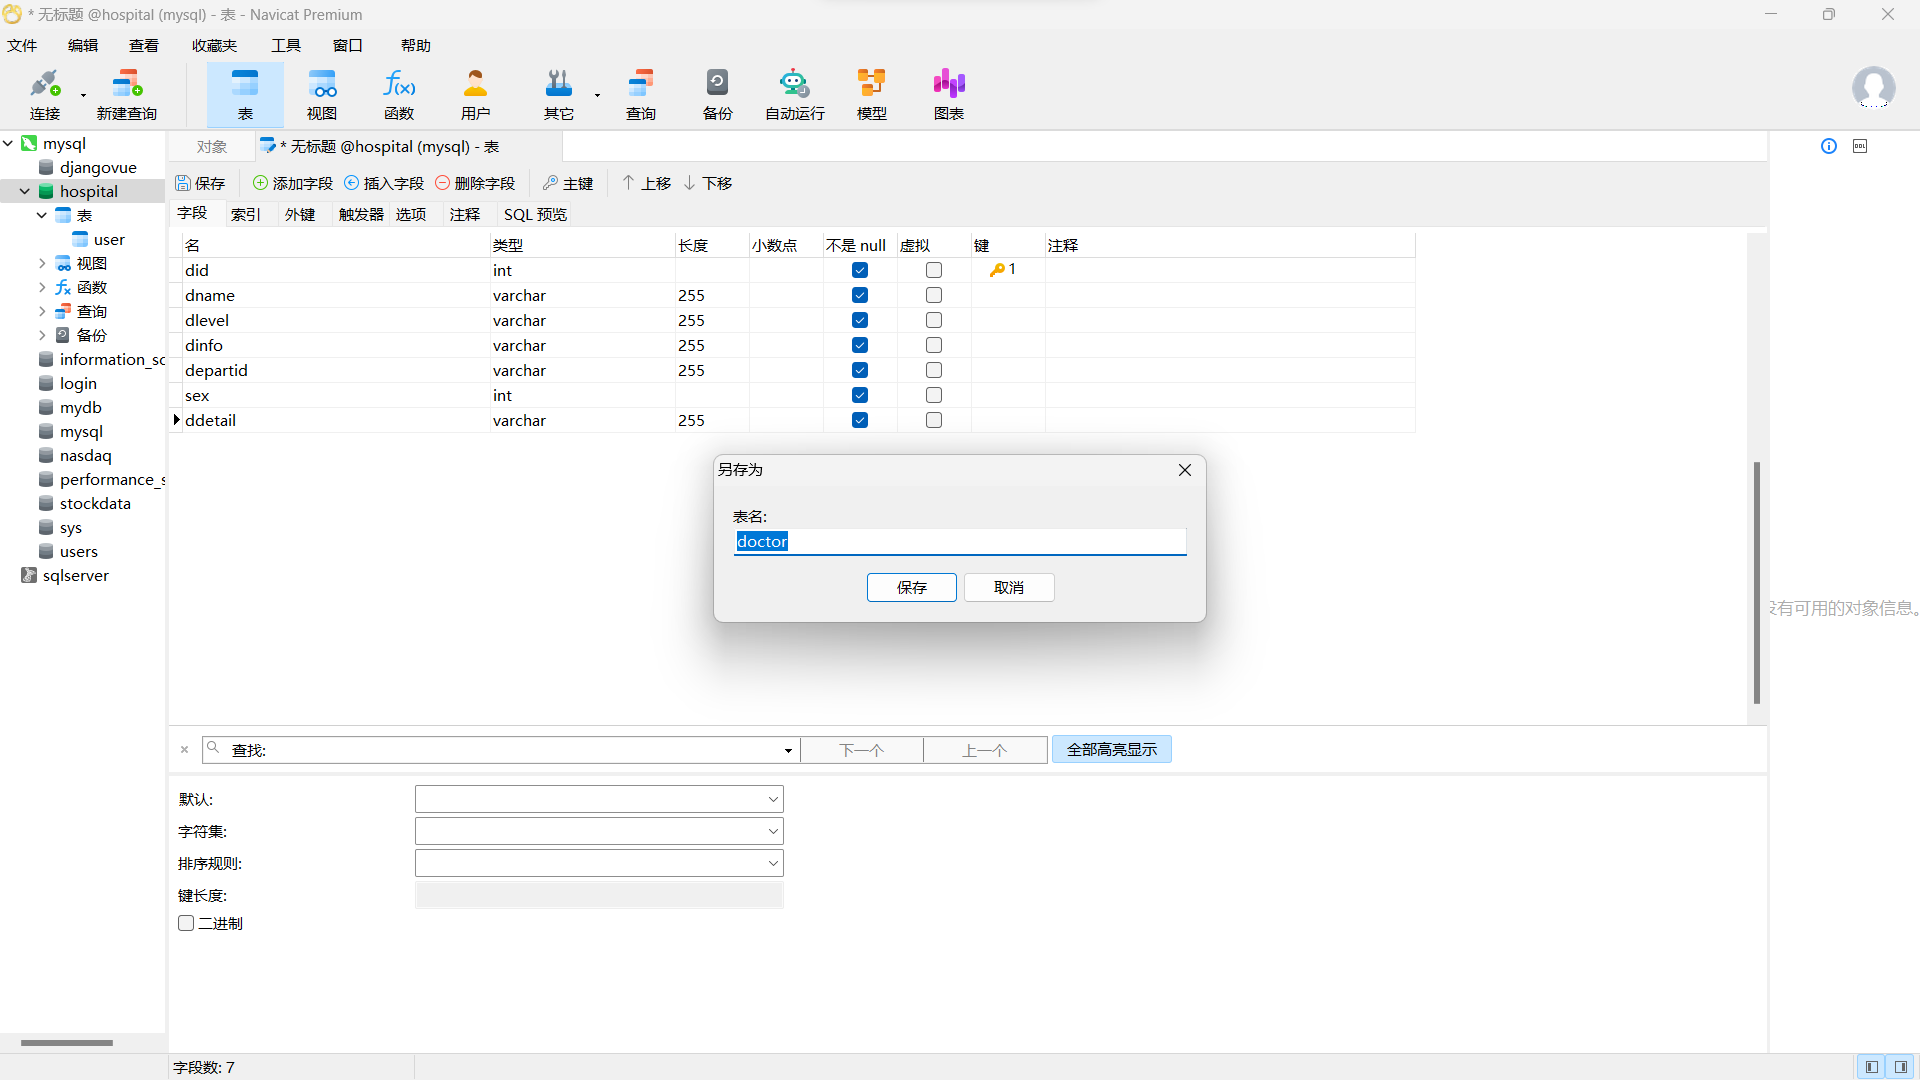
\includegraphics[width=0.9\textwidth]{imgs/6.png}
    \caption{doctor表}
\end{figure}

设计出的table结构如下

\begin{lstlisting}[frame=shadowbox]
+----------+--------------+------+-----+---------+-------+
| Field    | Type         | Null | Key | Default | Extra |
+----------+--------------+------+-----+---------+-------+
| did      | int(11)      | NO   | PRI | NULL    |       |
| dname    | varchar(255) | NO   |     | NULL    |       |
| dlevel   | varchar(255) | NO   |     | NULL    |       |
| dinfo    | varchar(255) | NO   |     | NULL    |       |
| departid | varchar(255) | NO   |     | NULL    |       |
| sex      | int(11)      | NO   |     | NULL    |       |
| ddetail  | varchar(255) | NO   |     | NULL    |       |
+----------+--------------+------+-----+---------+-------+
\end{lstlisting}

\subsubsection{depart表}

depart表的主要字段有departid,departname,分别代表科室id,科室名称

\begin{figure}[htbp]
    \centering
    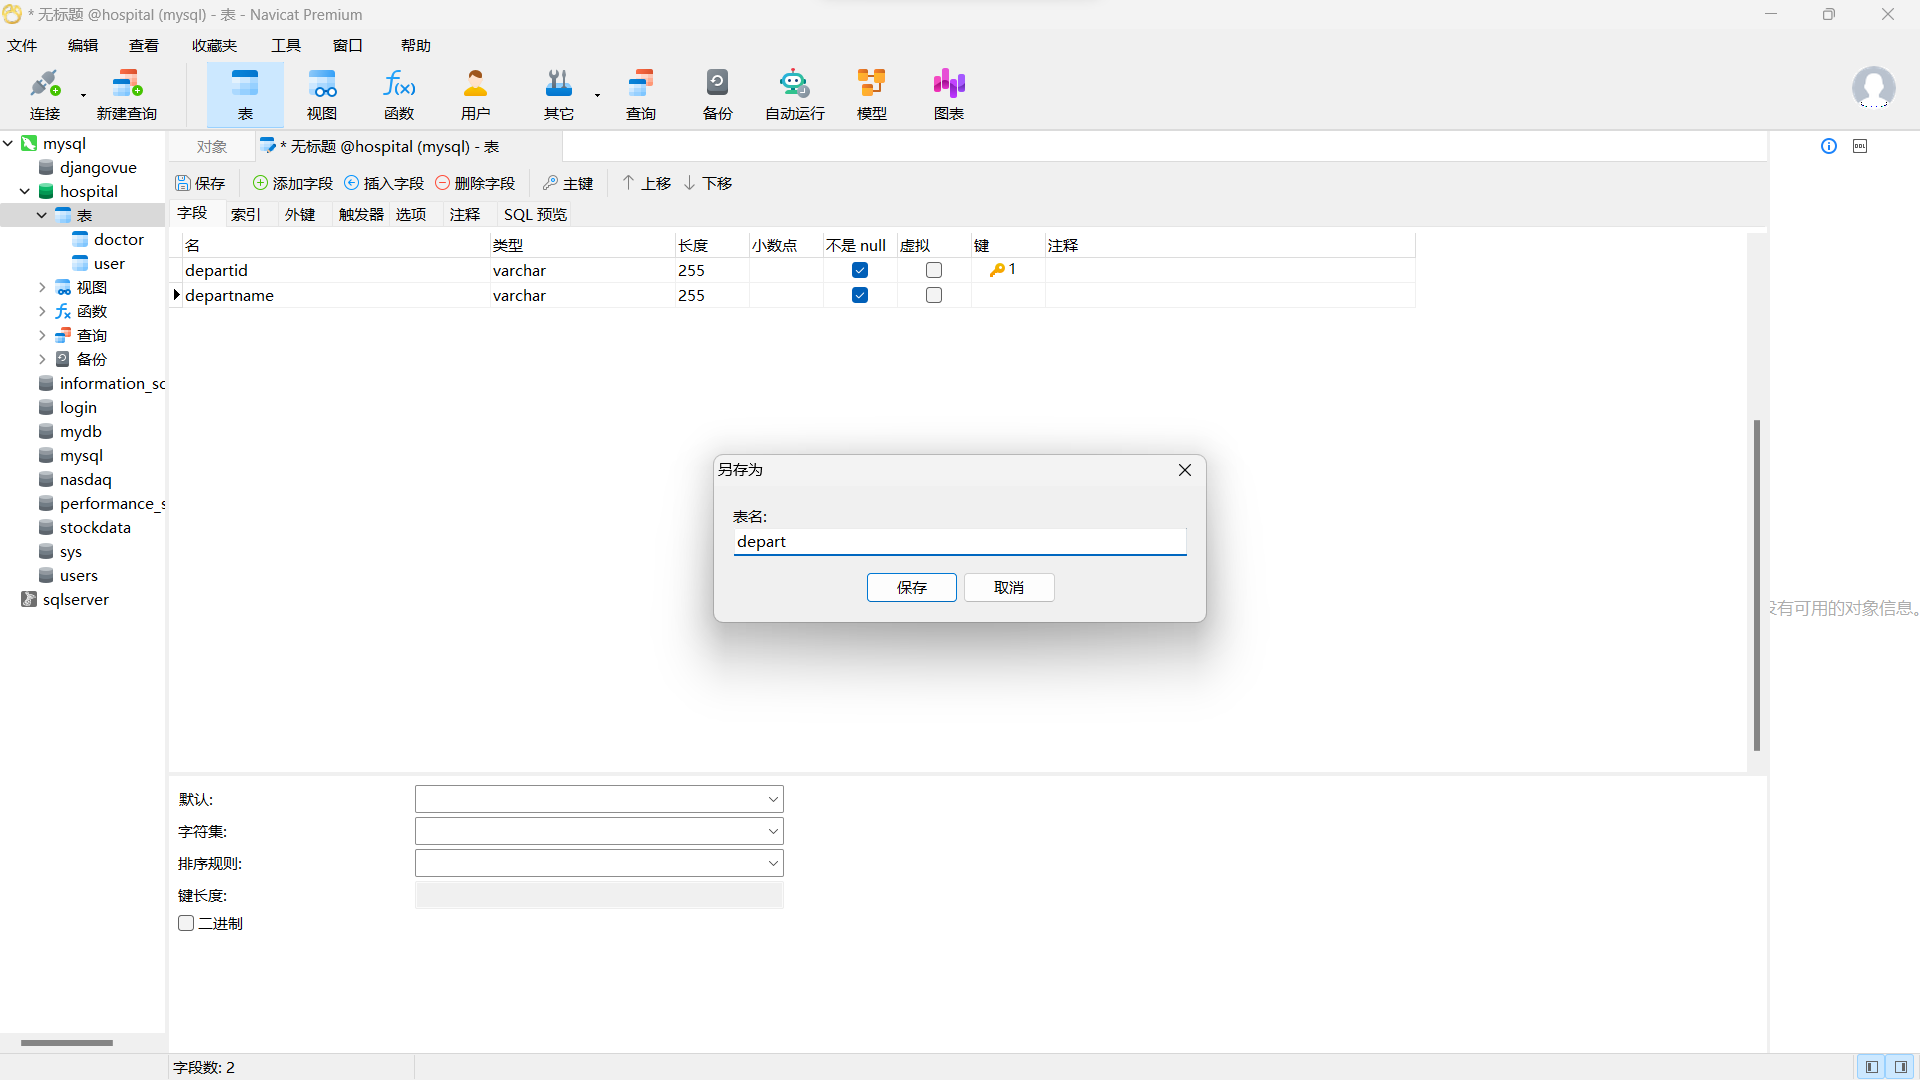
\includegraphics[width=0.8\textwidth]{imgs/7.png}
    \caption{depart表}
\end{figure}

设计出的table结构如下

\begin{lstlisting}[frame=shadowbox]
+------------+--------------+------+-----+---------+-------+
| Field      | Type         | Null | Key | Default | Extra |
+------------+--------------+------+-----+---------+-------+
| departid   | varchar(255) | NO   | PRI | NULL    |       |
| departname | varchar(255) | NO   |     | NULL    |       |
+------------+--------------+------+-----+---------+-------+
\end{lstlisting}

\subsubsection{schedule表}

schedule表的主要字段有sid,did,time,price分别代表排班id,医生id,排班时间,挂号费

\newpage

\begin{figure}[htbp]
    \centering
    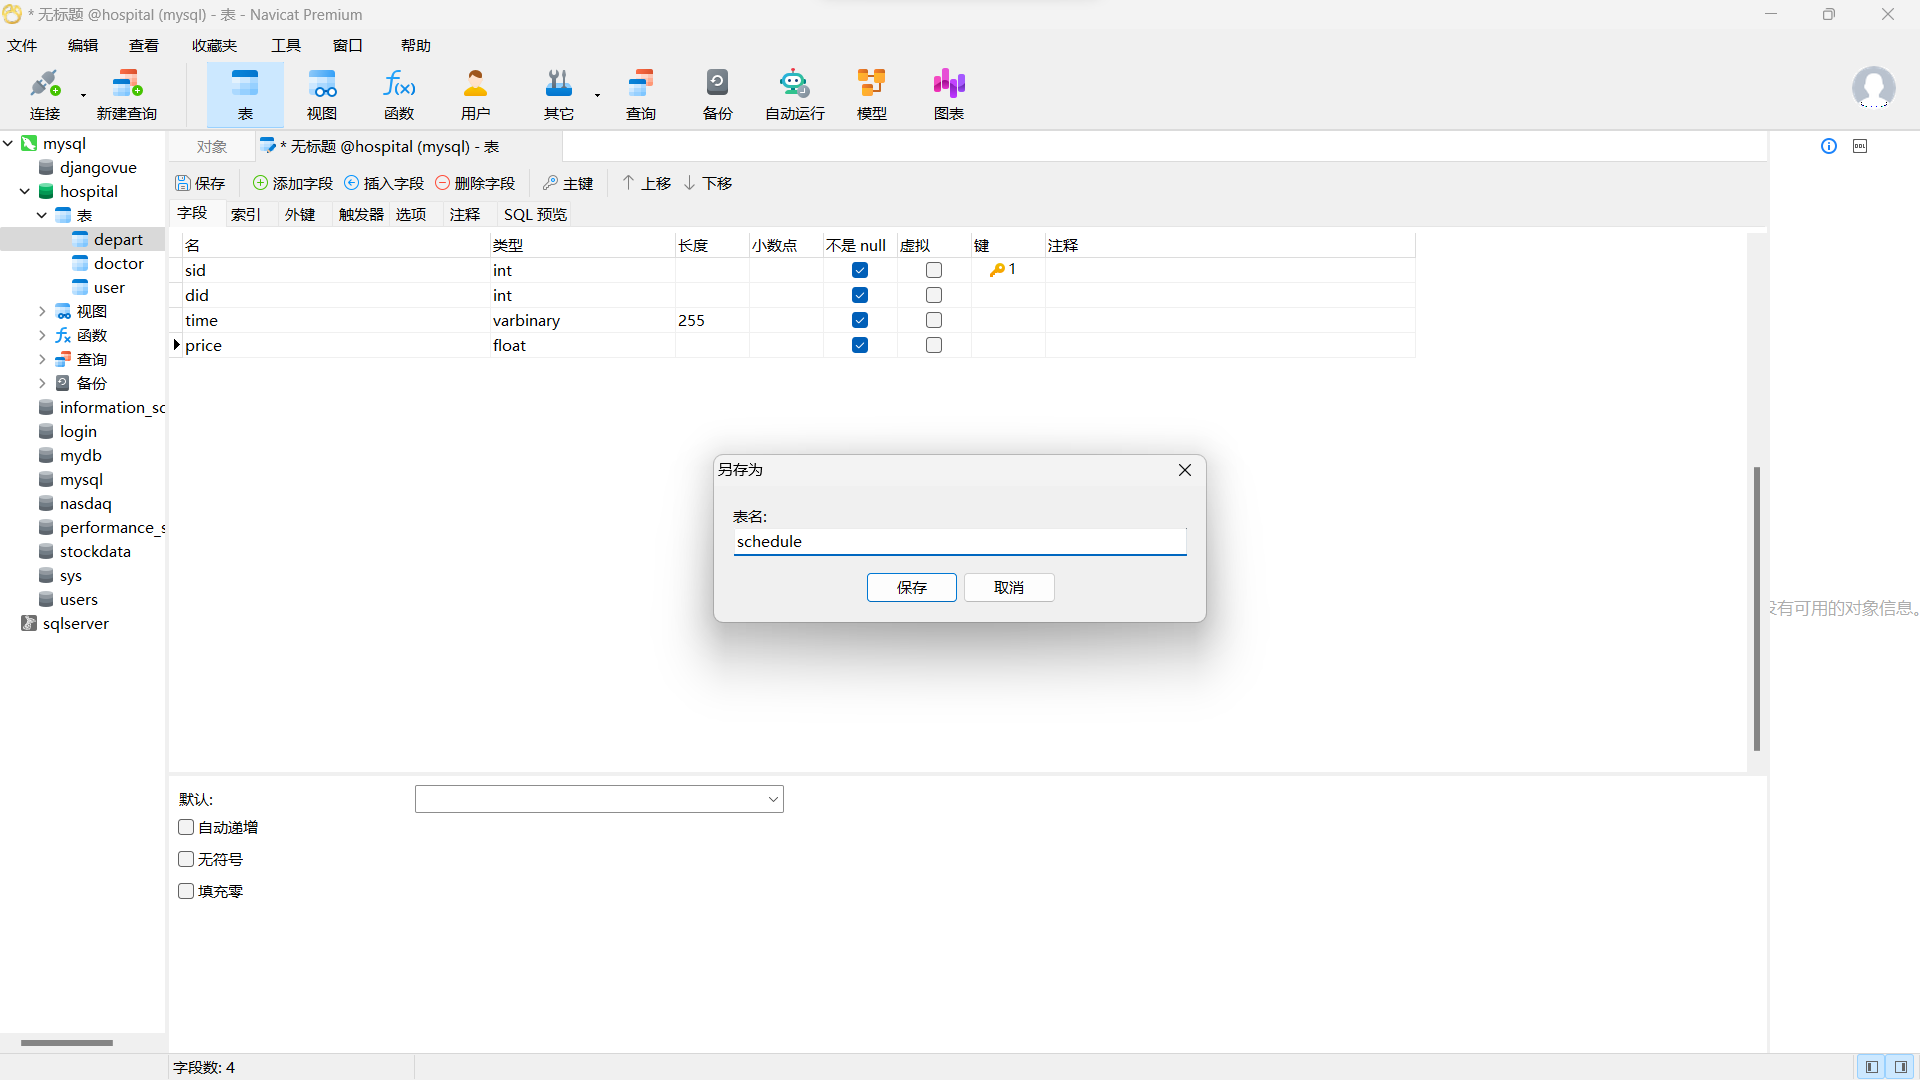
\includegraphics[width=0.8\textwidth]{imgs/8.png}
    \caption{schedule表}
\end{figure}

设计出的table结构如下

\begin{lstlisting}[frame=shadowbox]
+-------+----------------+------+-----+---------+-------+
| Field | Type           | Null | Key | Default | Extra |
+-------+----------------+------+-----+---------+-------+
| sid   | int(11)        | NO   | PRI | NULL    |       |
| did   | int(11)        | NO   |     | NULL    |       |
| time  | varbinary(255) | NO   |     | NULL    |       |
| price | float          | NO   |     | NULL    |       |
+-------+----------------+------+-----+---------+-------+
\end{lstlisting}

\subsubsection{myorder表}

myorder表的主要字段有oid,sid,did,分别代表订单id,排班id,医生id

\newpage

\begin{figure}[htbp]
    \centering
    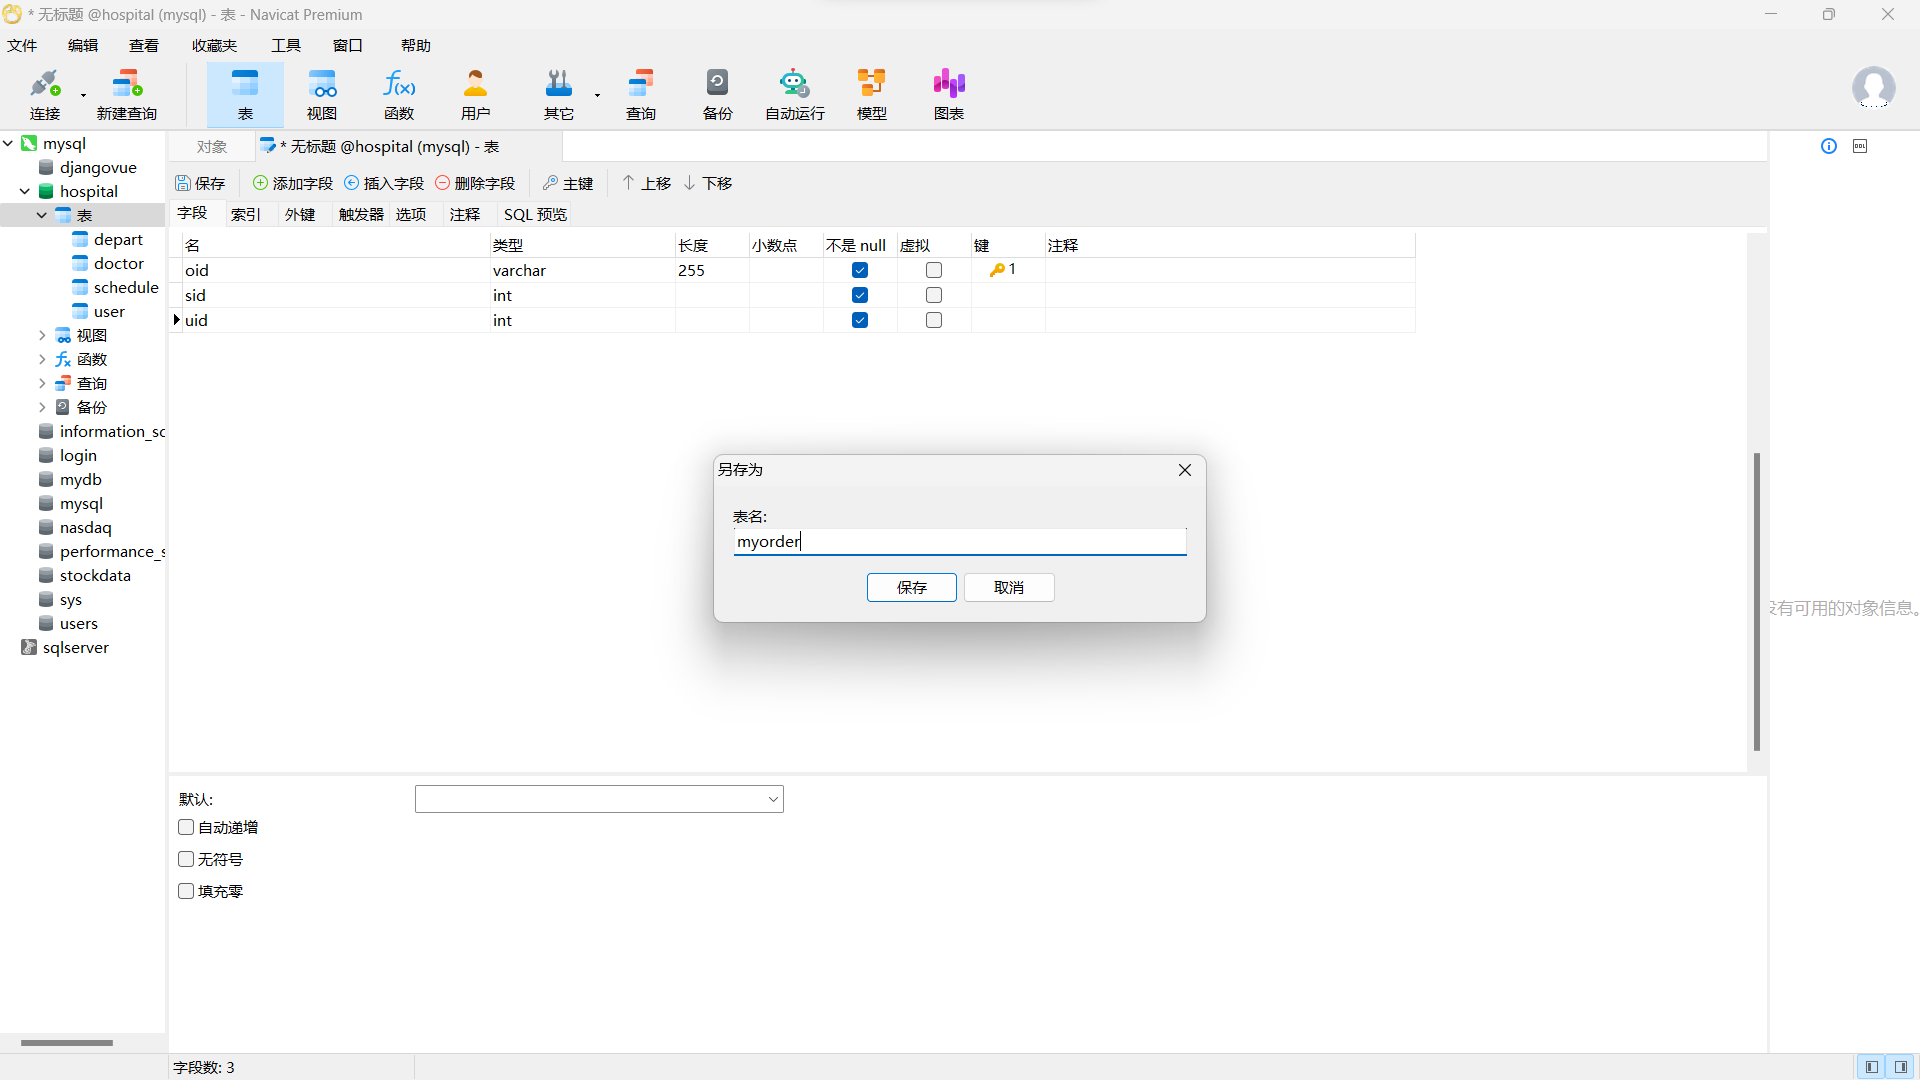
\includegraphics[width=0.8\textwidth]{imgs/9.png}
    \caption{myorder表}
\end{figure}

设计出的table结构如下

\begin{lstlisting}[frame=shadowbox]
+-------+--------------+------+-----+---------+-------+
| Field | Type         | Null | Key | Default | Extra |
+-------+--------------+------+-----+---------+-------+
| oid   | varchar(255) | NO   | PRI | NULL    |       |
| sid   | int(11)      | NO   |     | NULL    |       |
| uid   | int(11)      | NO   |     | NULL    |       |
+-------+--------------+------+-----+---------+-------+
\end{lstlisting}

\newpage

\subsection{Android看病预约客户端详细设计}

\newpage

\subsection{预约挂号Web服务器详细设计}

\newpage

\section{调试方法}

\newpage

\section{测试结果}

\newpage

\section{心得体会}

\newpage

\section{附录}

\newpage


\end{document}